\chapter{Resultat}
I denna del kommmer resultatet av projektet beskrivas. Det innebär dels
resultatet den mjukvara som har utvecklats, dels vilka erfarenheter som
teamet har samlat på sig under projektets gång.
\section{Systembeskrivning}
\textit{Skrivs när systemet är byggt, vill man få en känsla för hur det kan
komma att se ut så läser man bäst om det i arkitekturdokumentet}
\subsection{LoFi-Prototyper}
Under projektets andra iteration utvecklades tre olika LoFi-prototyper. Dessa
LoFi-prototyper designades för att visa på olika designalternativ på
användargränssnittet. Ett exempel på detta är informationen som var med i listan
över beslutade operationer. I en av prototyperna identifierades patienten som hörde ihop med beslutet med namn, den andra med personnummer. I den tredje LoFi-prototypen
fanns inget som identifierade patienten utan enbart information om vilken
typ av operation det var. På liknande sätt utvärderades olika sätt att
visualisera lediga tider i schemat samt olika sätt att anpassa sökparametrarna för en sökning efter lediga tider. När prototyperna visades för kunden kunde alternativen sållas bort och en tydligare bild av behoven framträdde.
Till exempel fanns det endast personnummer och inte namn på patienterna, vilket var något som önskades.

Den första iterationen av LoFi-prototyper användes sedan för att ta fram en ny
LoFi-prototyp med enbart mindre designalternativ som visades för tre olika
operationsplanerare.
\subsection{Systemanatomi}
\begin{figure}
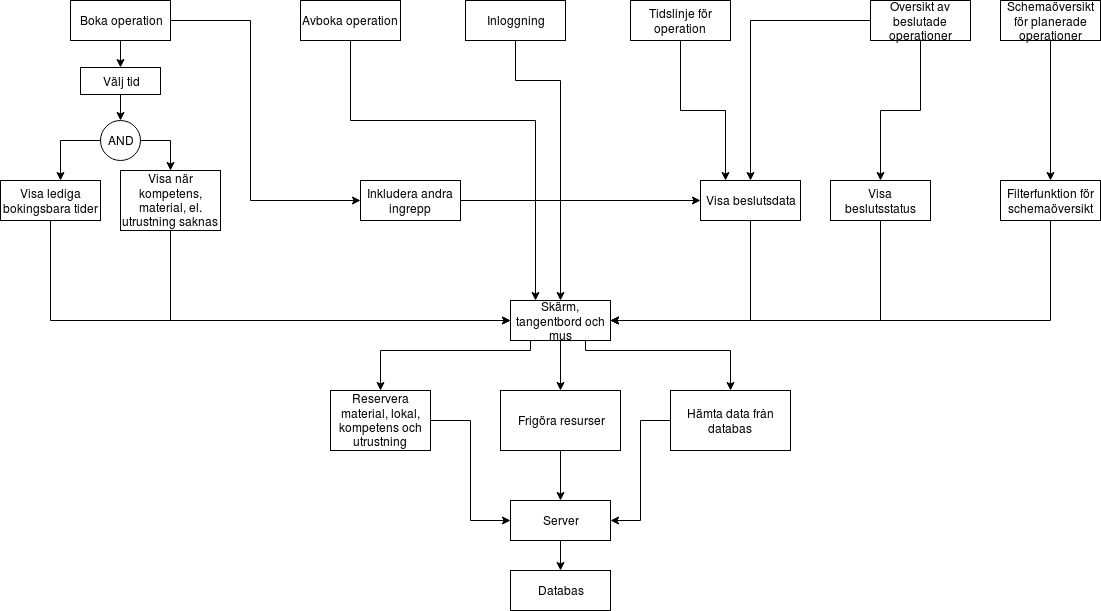
\includegraphics[width=\textwidth,height=.4\textheight]{Figures/Systemanatomi.png}\\
\caption{Systemanatomi}
\label{fig:Systemanatomi}
\end{figure}

I första iterationen togs det fram en systemanatomi som användes under projektets gång som ett hjälpmedel för strukturera upp arbetet under utvecklingen. Den gav en översiktlig bild av vilken funktionalitet produkten innehöll och hur de olika delarna samverkade med varandra. Utöver detta presenterades den i ett tidigt skede för kunden i syfte att säkerställa att projektgruppens syn på systemet stämde överens med kundens. 

\subsection{Värde för kund}
Den produkt som har skapats är ett lättöverskådligt schemaläggningssystem för operationer. Det följer ***Skriv in typiskt bra krav som är godkända av kund och som visar på funktionalitet och värde för kunden***

\section{Separation av front-end och back-end}

\section{Integration i redan existerande system}

\section{Gemensamma erfarenheter}
I början av projektet fick vi snabbt större erfarenhet av olika områden
tack vare de olika presentationer som de olika deltagarna i projektet gav.
Vi fick även en ökad förståelse för hur delar av sjukvården fungerar och att ett bra
it-system kan göra verklig skillnad.

\section{Översikt över individuella bidrag}
I denna delen presenteras deltagarnas individuella bidrag översiktligt.

\todo{Lägg till era rubriker och en kort synopsis här}
\subsection{Adam}
En studie i hur teamledarens roll går att applicera tillsammans med scrum-metodik.
\subsection{Björn}
Hur kan versionshantering användas effektivt för ett mindre mjukvaruutvecklings projekt.
\subsection{Christoffer}
Betydelsen av att samla krav från en varierad grupp aktörer
\subsection{Henrik}
För/nackdelar med TypeScript jämfört med JavaScript
\subsection{Martin}
Angular som webbutvecklingsplattform
\subsection{Niclas}
Pappersprototypens betydelse vid utveckling av programvara
\subsection{Tor}
Kvalitetsförsäkrande metoder i ett småskaligt mjukvaruprojekt
